\section{Highspeed Digital Design}

\subsection{Timing Analysis}
Goal: to check whether the timing specifications are met.

\begin{table}[htbp]
    \centering
    \begin{tabularx}{0.8\linewidth}{lX}
        static (STA) & calculates timing without simulations \\
            & always covers extremes \\
         dynamic & is a timing simulations \\
             & may fail to find longest path \\
    \end{tabularx}
\end{table}

Note that STA is not able to cover interfaces between different clock regions!

\begin{multicols}{2}
    Consider four types of paths:
    \begin{enumerate}
        \item clock-to-clock 
        \item input-to-clock
        \item clock-to-output
        \item input-to-output
    \end{enumerate}
    \vfill
    \columnbreak
    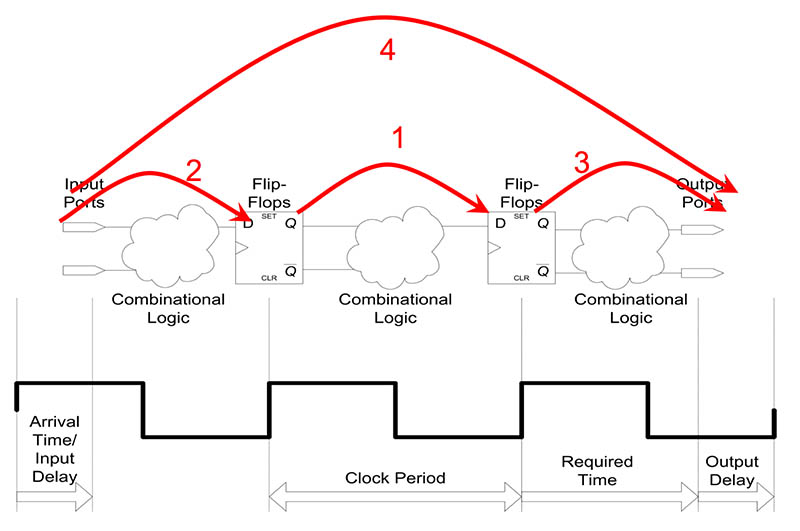
\includegraphics[width=0.8\linewidth]{images/HSDigital_TimingAnalysis.jpg}
    %TODO: draw nice picture in TikZ
\end{multicols}

Consider: minimum / maximum delays, dependence on voltage, temperature, process, load, edge (rising/falling)

\paragraph{Clock-to-clock}The maximal path consists of 
\begin{itemize}
    \item $t_{PCQ}$: max. clock-to-output delay of flip-flop
    \item $t_{NET}$: max. data path between flip-flops
    \item $t_{SETUP}$: max. data setup time to clock of second flip-flop 
\end{itemize}

Static timing analysis on base of a schematic assumes standard net lengths (a 2-pin net is assumed to be shorter than a 3-pin net, etc.).

\begin{multicols}{2}
    \begin{tikztimingtable}
    Basic Clock              & LLHHHHHHHHLLLLLLLL \\
    Flip-Flop 1 Clock    & LLLHHHHHHHHHLLLLLL \\
    Flip-Flop 2 Clock    & LLLLLLLLLHHHHHHHHL \\
    \extracode
    \draw[blue,->] (3,-1.8) to[out=0,in=180] (9,-3.4);
    \node at (7,-2) {\color{blue}$t_{PATH}$};
\end{tikztimingtable} \\
    \vfill
    \columnbreak
    The maximal path must be shorter than the clock period (plus the delay from the clock source to the second flip-flop, minus the delay from the clock source to the first flip-flop)
\end{multicols}

%TODO: maybe add example?

\paragraph{Delays}There exist two types of delay: \emph{gate} delays and \emph{wire} delays. \\
\begin{table}[htbp]
    \centering
    \begin{tabularx}{0.8\linewidth}{XX}
        Gate delays & Wire delays \\ \toprule
        \begin{circuitikz} \draw (0,0) node[not port] {} (1,0); \end{circuitikz}
        & \tikz[scale=0.5]{\draw (0,0)--(1,0)--(1,1)--(2,1) (1,0)--(1,-1)--(2,-1)--(2,-0.5)--(3,-0.5) (2,-1)--(2,-1.5)--(3,-1.5); \draw[fill=black] (1,0) circle (0.1) (2,-1) circle (0.1);}  \\
        through transistors, semiconductors & through wires \\
        dependent on:  \newline
        - temperature (higher $\to$ higher delays)\newline
        - voltage (higher $\to$ lower delays)\newline
        - technology, load, \dots
        & dependent on:\newline
        - length of wire \newline
        - resistance, capacitance, inductance \newline
        - low dependency on temperature \\
        \bottomrule
    \end{tabularx}
\end{table}

\paragraph{Conditions}Commercial: BCC (Best case Commercial) is the fastest, WCC (Worst Case Commercial) is the slowest case. Other conditions: Industrial (BCI, WCI), Military (BCM, WCM) \\

\paragraph{Multi clock cycle path}A combinatorial which takes more time than one clock cycle. 
Problem: you do not always know, when the signal arrives at the output. 
Solution: e.g. define \emph{clock enable} signal and latch only e.g. every fourth input to the logic part and the output.

\paragraph{False path}A path which physically exists, but is never used, e.g.
\begin{itemize}
    \item Two MUX in series, not all paths are logically possible
    \item False path to define a relation between two asynchronous clocks
    \item Test logic, which would not run at full speed and is not optimized for speed.
\end{itemize}

\subsection{Timing Simulation}
\paragraph{Cycle based simulation}
Events only happen at clock edges, thus no delays are considered.
Cycle based simulation is purely \emph{functional}.
\paragraph{Unit delay simulation}
Assumes a standard delay, which leads to a simple model. Not very relevant.
\paragraph{Prelayout timing simulation}
Uses propagation times from data sheets and standard values.
\paragraph{Postlayout timing simulation}
Uses actual wire geometries, including parasitics.
By far the slowest, but the only really accurate timing simulation.

\subsection{Clock Distribution Schemes}

\paragraph{Common-clock distribution timing}
Common (third-party) clock used by driver and receiver. OK for up to \SI{200}{\mega\hertz}. 

\paragraph{Source synchronous / Incident}
Driver sends clock and data. 
Source synchronous: driver delays data slightly. 
Incident clocking: receiver delays data.

\paragraph{Embedded clocking}
Clock is embedded in data (e.g. Manchester coding).
Saving on number of lines, but increase of frequency.